%! TEX program = pdflatex

\documentclass[11pt]{article}
\usepackage{polski}
\usepackage{tgpagella}
\usepackage{hyperref}
\usepackage{graphicx}
\usepackage{caption}
\usepackage{subcaption}
\usepackage{amsmath}
\usepackage{amsfonts}
\usepackage{booktabs}
\usepackage{rotating}
\usepackage{array}
\usepackage{multirow}
\usepackage{amsthm}
\usepackage{mdframed}
\usepackage[explicit]{titlesec}

\usepackage[
	left=1in, right=1in, top=.5in, bottom=.5in
]{geometry}

\hypersetup{
colorlinks=true,
urlcolor=blue
}

\graphicspath{
	{../graphics/}
}

\newmdtheoremenv{definition}{Definicja}


\author{Emil Olszewski, Artur Sadurski}
\date{\today}
\title{Prognozowanie popytu na energię elektryczną na amerykańskim rynku day-ahead. \\ \large Komputerowa analiza szeregów czasowych \\ \large Raport 2. }


\begin{document}
\maketitle

% ------------------- STRESZCZENIE --------------------------
\begin{abstract}
Poniższy raport przedstawia analizę szeregu czasowego opisującego obciążenie na sieci elektrycznej na podstawie danych z rynku amerykańskiego z przestrzeni dni od 01.01.2016 do 31.12.2017. Celem raportu jest dopasowanie modelu ARMA do danych, a następnie predykcja zapotrzebowania w przyszłości. Predykcja taka jest istotna dla operatorów sieci, którzy muszą dostosować produkcję energii do zapotrzebowania. W pierwszej części raportu przedstawiono wstęp teoretyczny dotyczący rynków day-ahead, szeregów ARMA oraz opisano dane i ich charakterystykę. 
\end{abstract}

% ============================================================
% =========               WSTĘP                      =========
% ============================================================
\section{Wstęp}

% ---------------- RYNKI DAY-AHEAD --------------------------
\subsection{Rynki day-ahead} 

W przypadku energii elektrycznej do zawierania kontraktów kupna-sprzedaży pomiędzy spółkami energetycznymi a operatorami elektrowni i sieci dochodzi na rynku \textit{day-ahead}, który nie pozwala na ciągły handel między uczestnikami. Na taki rynek spływają oferty kupna i dostarczenia konkretnej ilości energii na \textbf{każdą godzinę następnego dnia}. Ceny na każdy z tych okresów wyznaczane są jako punkt przecięcia się \textbf{krzywej popytu} i \textbf{podaży}. 

% ----------------- SZEREGI ARMA ----------------------------
\subsection{Szeregi ARMA}
Głównym celem raportu będzie dopasowanie szeregu ARMA do danych, więc należy wpierw przypomnieć jego definicję. 

\begin{definition}

Szereg czasowy ${\left\lbrace X_t \right\rbrace}_{t \in \mathbb{Z}}$ nazywamy szeregiem $\text{ARMA}(p, q)$ gdy da się go przedstawić jako

$$ X_t = \varepsilon_t + \sum_{i=0}^p \phi_i\,X_{t-i} + \sum_{i=0}^q \theta_i\,\varepsilon_{t-i} $$

gdzie współczynniki $\phi_i$ oraz $\theta_i$ to współczynniki modelu zaś $\varepsilon_i \sim \text{WN}(0, \sigma^2)$. 

\end{definition}


% ---------------- OPIS DANYCH -------------------------------
\subsection{Opis danych}
\href{https://www.kaggle.com/datasets/robikscube/hourly-energy-consumption}{Dane}, do których został dopasowany model zostały udostępnione w domenie publicznej. Przedstawiają one ilości energii elektrycznej na którą zostały zawarte kontrakty na rynku \textbf{PMJ} na każdą godzinie dni pomiędzy 01.01.2016 a 31.12.2017. Obejmują więc okres dwuletni. Horyzont czasowy specjalnie został dobrany tak aby można było zaobserwować różne sezonowości dotyczące cen energii elektrycznej, to jest \textbf{sezonowość dobową} (związaną z cyklem dzień-noc), \textbf{tygodniową} (dni robocze-weekend) oraz \textbf{roczną} (pory roku). Przykładowe trajektorie przedstawiono na rysunku \ref{fig:trajektorie}.


\begin{figure}[h!]
    \centering
    % Top plot
    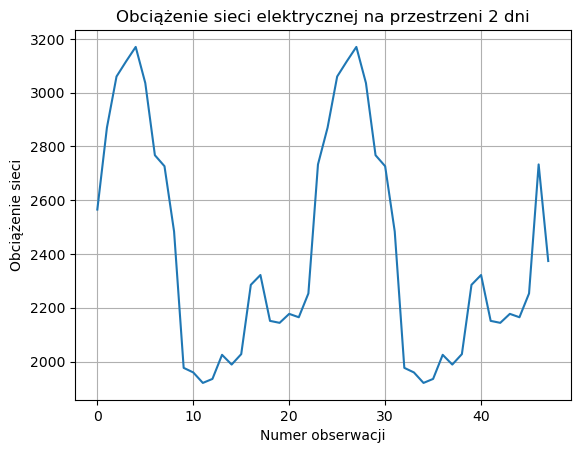
\includegraphics[width=0.45\textwidth]{../plots/dane_dwudniowe.png}
    
    % A little vertical space between the rows of images
    \vspace{1cm}

    % Bottom left plot
    \begin{minipage}[b]{0.45\textwidth}
        \centering
        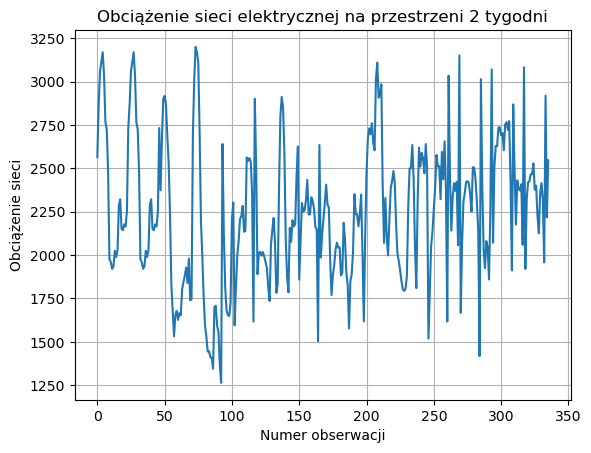
\includegraphics[width=\textwidth]{../plots/dane_dwutygodniowe.png}
    \end{minipage}
    \hfill
    % Bottom right plot
    \begin{minipage}[b]{0.45\textwidth}
        \centering
        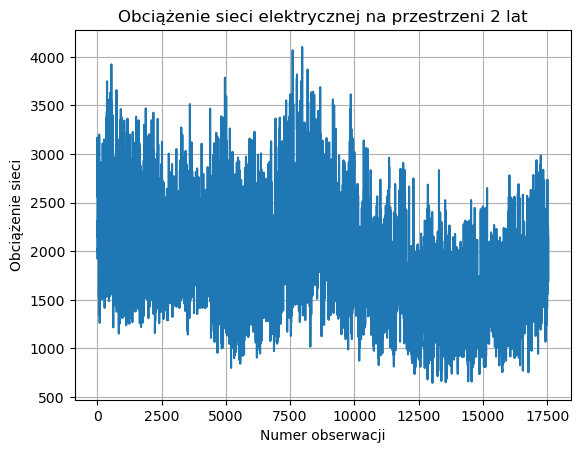
\includegraphics[width=\textwidth]{../plots/dane_dwuletnie.png}
    \end{minipage}
	\caption{Trajektorie popytu na energię elektryczną przedstawione w różnych rozdzielczościach czasowych.}
	\label{fig:trajektorie}
\end{figure}


% ----------------- ANALIZA DANYCH ---------------------------
\section{Analiza danych}

\subsection{Stacjonarność}

\begin{figure}[h!]

	\centering
	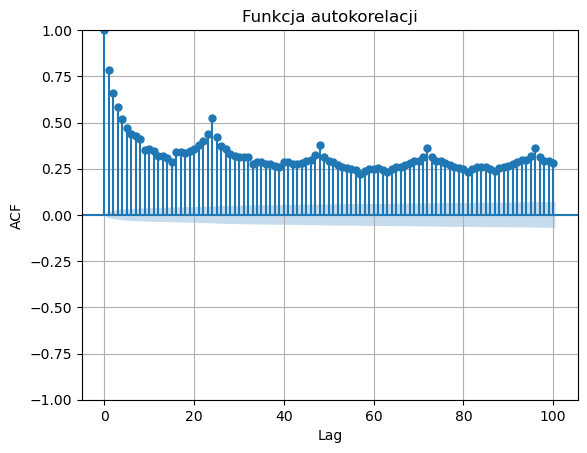
\includegraphics[width=0.45\textwidth]{../plots/acf_niezmodyfikowane.png}
	\hfill
	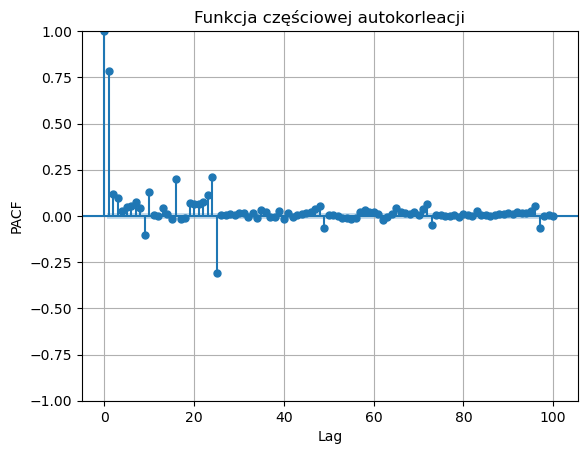
\includegraphics[width=0.45\textwidth]{../plots/pacf_niezmodyfikowane.png}
	\caption{Wykresy ACF i PACF wskazują na to, że szereg nie jest stacjonarny.}
	\label{fig:acf_pacf_niezmodyfikowane}

\end{figure}

Zaczniemy od przebadania danych pod względem ich stacjonarności. Własność ta jest kluczowa aby efektywnie dopasować model ARMA. Wpierw użyjemy \textbf{funkcji autokorelacji} oraz \textbf{częściowej autokorelacji}, więc przypomnijmy ich definicje. \\

\begin{definition}
\textbf{Funkcja autokorelacji (ACF)} dla szeregu czasowego ${\left\lbrace X_t \right\rbrace}_{t \in \mathbb{Z}}$ to funkcja $\rho$ określona wzorem 
$$ \rho(k) = \frac{\gamma\left(k\right)}{\gamma\left(0\right)} $$
gdzie $\gamma(k) = \text{Cov}(X_t, X_{t-k})$ to funkcja autokowariancji.
\end{definition}

\begin{definition}
\textbf{Funkcja częściowej autokorelacji (PACF)} dla szeregu czasowego ${\left\lbrace X_t \right\rbrace}_{t \in \mathbb{Z}}$ to funkcja $\alpha$ określona równaniami 
$$ \alpha\left(0\right) = 1$$ 
oraz 
$$ \alpha\left(k\right) = \phi_{kk}, $$
gdzie $\phi_{kk}$ to ostatnia współrzędna wektora $\phi_k$ danego wzorem 
$$ \phi_k = \Gamma_k^{-1}\gamma_k, $$
$ \Gamma_k = \left[\gamma\left(i - j\right)\right]_{i,j = 1}^k $, $\gamma_k = \left[\gamma\left(1\right), \gamma\left(2\right), \ldots, \gamma\left(k\right)\right]$.
\end{definition}

Na wykresach \ref{fig:acf_pacf_niezmodyfikowane} przedstawiono wykresy próbkowych ACF i PACF dla poszczególnych przesunięć czasowych. Jak widać funkcja autokorelacji nie zanika do zera, co byłoby charakterystyczne dla szeregu ARMA, lecz oscyluje wokół pewnej wartości. Choć od pewnego momentu funkcja PACF wydaje się zanikać do zera, to możemy zaobserwować okresowo występujące wartości odstające. Wszystko to wskazuje, że nie mamy do czynienia ze stacjonarnym szeregiem czasowym.
\end{document}